\documentclass[rep.tex]{subfiles}
\begin{document}

\chapter{Zadanie 4}
\label{zad4}
\section{Treść}
Zaprojektować symetryczną linię paskową, rys.~\ref{fig:zad4:stripline},
o impedancji charakterystycznej~$Z_0 = 50~\Omega$.
Podłoże linii stanowi dielektryk o $\epsilon_r = 2.56$, $\mu_r = 1$ i grubości $b = 2.8~mm$.
Obliczenia wykonać, przy założeniu, że grubość przewodu wewnętrznego~$t = 0~mm$.
Metodą różnic skończonych obliczyć impedancję charakterystyczną tej linii przyjmując,
że przewód wewnętrzny~$t = 0.150~mm$.

\begin{figure}[!htbp]
  \centering
  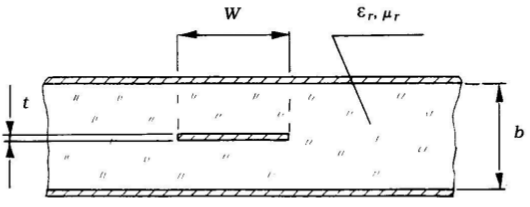
\includegraphics[scale=0.5]{fig/zad4/stripline}
  \caption{Symetryczna linia paskowa}
  \label{fig:zad4:stripline}
\end{figure}

\section{Rozwiązanie}
\subsection{Nieskończenie cienki przewód wewnętrzny}
\label{zad4:thin}
Impedancja charakterystyczna symetrycznej linii paskowej wyraża się wzorem:
\begin{equation}
  Z_0(k) = 29.976 \pi \sqrt{\frac{\mu_r}{\epsilon_r}} \frac{K(k)}{K'(k)} \label{eqn:zad4:z}
\end{equation}
gdzie:
\begin{equation}
  k = \frac{1}{\operatorname{ch}\,(\frac{\pi w}{2b})} \label{eqn:zad4:k}
\end{equation}
przy założeniu nieskończenie cienkiego paska~($t = 0~mm$).
Z równania~\ref{eqn:zad4:k} można wyznaczyć szerokość paska:
\begin{equation}
  w = \frac{2b}{\pi} \ln\big(\frac{1}{k} + \sqrt{\frac{1}{k^2} - 1}\big) \label{eqn:zad4:w}
\end{equation}
która to tworzy linie o impedanacji~$Z_0$.

W pierwszym kroku z równania~\ref{eqn:zad4:z} można wyznaczyć stosunek całek eliptycznych $\frac{K(k)}{K'(k)}$:
\begin{equation}
  \frac{K(k)}{K'(k)} = \frac{Z_0}{29.976 \pi}\sqrt{\frac{\epsilon_r}{\mu_r}}. \label{eqn:zad4:modk}
\end{equation}
Następnie można wyznaczyć stałą modularną~$q$:
\begin{equation}
  q = e^{- \pi \frac{K'(k)}{K(k)}}. \label{eqn:zad4:modq}
\end{equation}
Stała modularna z równania~\ref{eqn:zad4:modq} pozwala wyznaczyć wartość szeregów:
\begin{align}
  N &= \sum_{i=1}^\infty q^{i \times (i-1)}, \label{eqn:zad4:N} \\
  D &= 0.5 + \sum_{i=1}^\infty q^{i \times i}. \label{eqn:zad4:D}
\end{align}
Szeregi~\ref{eqn:zad4:N} i~\ref{eqn:zad4:D} są szybko zbieżne i wystarczy już kilka pierwszych wyrazów aby uzyskać dobrą dokładność.
W programie obliczanie wartości~$N$ oraz~$D$ zatrzymuję się automatycznie gdy osiągnięta została dokładność,
która jest podawana jako parametr funkcji.

Korzystając z wyznaczonych wartości można obliczyć moduł~$k$:
\begin{equation}
  k = \sqrt{q} \Big(\frac{N}{D}\Big)^2.
\end{equation}

Podstawiając wartość do równania~\ref{eqn:zad4:w} można obliczyć wymaganą szerokość paska.
Dla danych podanych w treści zadania wymagana wartość $w = 2.06265925327~mm$.

\subsection{Przewód wewnętrzny o $t = 0.150~mm$}
\label{zad4:thick}
W celu obliczenia dokładniejszej wartości impedancji skorzystano z metody różnic skończonych.
W tym celu należy wyznaczyć rozkład potencjału w linii.
Wykorzystano w tym celu algorytm Liebmanna opisany w~\cite{num}.
Wynik został przedstawiony na rys.~\ref{fig:zad4:u}.

\begin{figure}[!htbp]
  \centering
  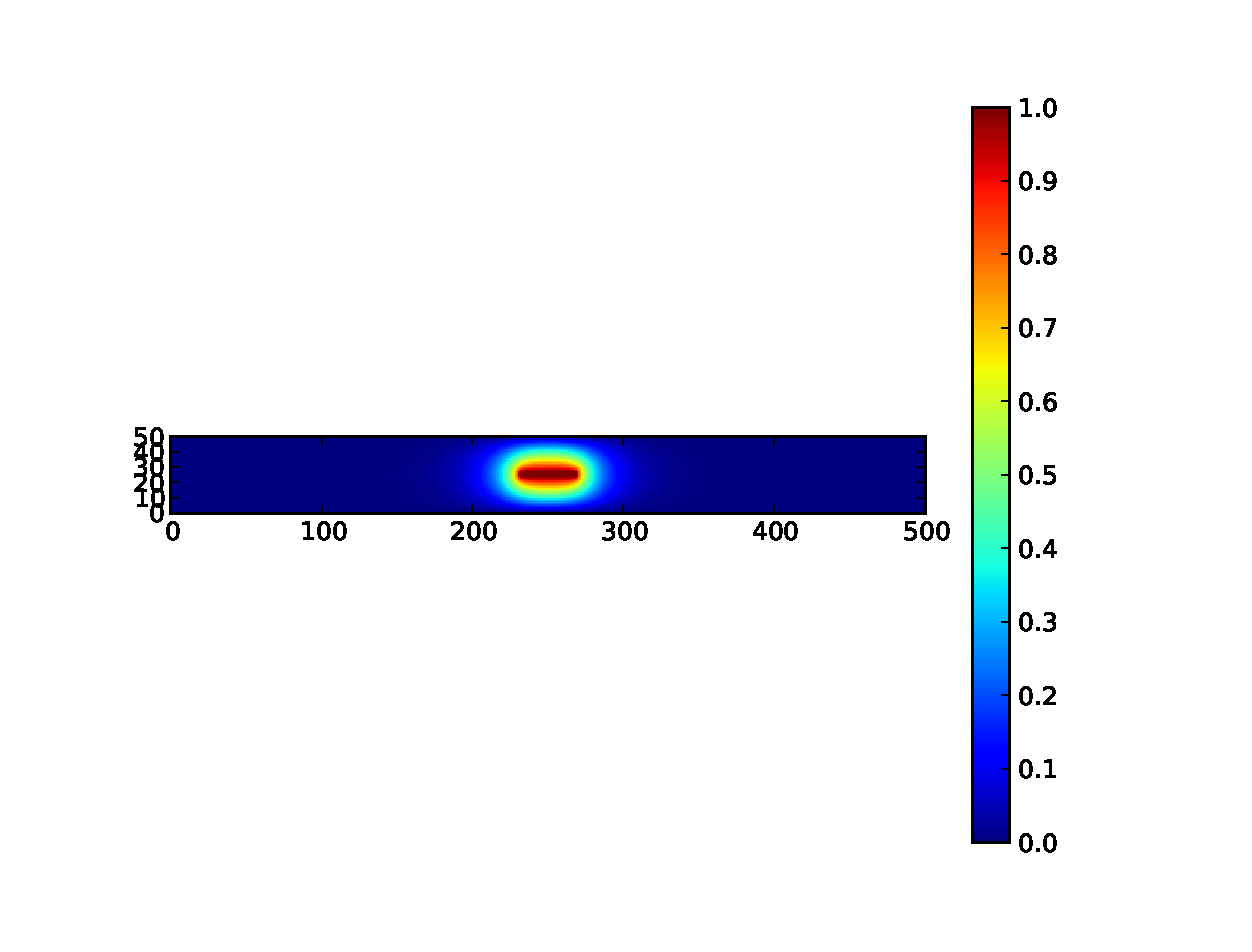
\includegraphics[scale=0.5]{fig/zad4/u}
  \caption{Rozkład potencjału w symetrycznej linii paskowej}
  \label{fig:zad4:u}
\end{figure}

Mając dany rozkład potencjału możemy obliczyć impedancję linii:
\begin{equation}
  \label{eqn:zad4:imp}
  Z_0 = \sqrt{\frac{\mu}{\epsilon}}\frac{U}{\oint_{S_2}E_n\mathrm{ds}}
\end{equation}
gdzie $U$ to napięcie pomiędzy przewodem wewnętrznym a zewnętrznym,
$E_n$~to składowa normalna natężenia pola elektrycznego określona na linii brzegowej~$S_2$ przewodu zewnętrznego.

W wyniku symulacji uzyskano impedancję równą~$Z_0 = 45.2925852199~\Omega$,
dla przewodu o wymiarach określonych w sekcji~\ref{zad4:thin}.
Daję to różnicę równą~$4.70741478~\Omega$ od wymaganych~$50~\Omega$.
\end{document}
